% !TEX root = 99_main.tex

The experiment, consisting of 15 users each equipped with a fitbit over a month, produced a dataset of 1460 data points. Each data point is effectively a survey of the user at a particular time. The results presented in this section is a demonstration of the type of analysis that can be conducted using data acquired from the cozie watch-face.

\subsection{Overview of spatial temporal data}

Figure \ref{fig:summary}a details the spatial distribution of data throughout Singapore. Each of these data points is tagged with the users heart-rate, response, and local temperature which can be used to infer faults or issues within the building. Figure \ref{fig:summary}b is a simple heatmap plotting the number of responses based on the hour of the day, and day of the week. It is interesting to note that there are more responses in the hours of 9:00, 11:00, 13:00, 15:00, and 17:00 when the occupant is buzzed and forced to give feedback. Nevertheless there are still significant amounts of responses made outside these times through the motivation of the participants themselves. Figure \ref{fig:summary}c details the daily responses from the participants, and no observable decrease in responses can be made. Dips in responses naturally occur during the weekend. A normal distribution of heart-rate data from the fitbit heart rate sensor can be found in Figure \ref{fig:summary}d. 




\subsection{Combination with external sensor data}

Combining the cozie watch face, with additional environmental sensors opens further dimensions of analysis. User responses are mapped to the environmental condition at which they are exposed to, which can provide a high quality labeled data set for training data driven models. Figure \ref{fig:summary}e-f detail the distribution of temperature and humidity data. Unfortunately, due to communication issues from these sensors, not all data points could be recorded. The temperature of the temperature sensor, is on average 0.8 $^\circ$C warmer than the surrounding environment due to the influence of body temperature. 




\begin{figure}
\begin{center}
\includegraphics[width=\textwidth, trim= 0cm 0cm 0cm 0cm,clip]{cozie_datasummary.pdf}
\caption{Overview of raw data extracted from the cozie watch face and additional sensors. (a) spatial distribution of responses throughout Singapore, (b) temporal distribution of responses, (c) number of responses per day over the course of the experiment, (d-f) normalised distribution of responses based on the fitbit heart rate sensor, wrist mounted temperature sensor, and of-body humidity sensor }
\label{fig:summary}
\end{center}
\end{figure}



\subsection{Influence of individual users}
\label{ch:userResults}

Individual user feedback can be clustered using un-supervised learning techniques. In this example, we use a hierarchal k-means clustering based on euclidean distance using the Nearest-Point-Algorithm. The results, shown in Figure \ref{fig:clustering}, show four distinct clusters of users. 
%Users that are comfortable 100\% of the time, users that are comfortable 60-80 \% of the time, those that are comfortable 50\% of the time and generally would prefer it cooler, those that are comfortable 50\% of the time and would prefer it both warmer and cooler. 
Understanding and defining these differences in user preferences can be used to recommend spaces that may better suit the needs of the occupant. For example, Group A, which seems to primarily be working off-site can be recommended alternative work spaces that are on average cooler. Group C on the other hand is a single highly satisfied user, who works from a single work-space within a narrow temperature range, and relatively low resting heart-rate. Group D represents our conventional occupant that may be comfortable 70\% of the time. 

Below the cluster plot are spatial distributions of responses that can be used to identify different building climates. The majority of "Prefer Warmer" responses occur in co-working space 1. This area can be labeled as a "cooler working space" for users that would prefer cooler working environments. Alternatively, if facilities management wishes to save energy, increasing the set-point temperature of these "over-cooled" spaces may be a low effort solution which may simultaneously improve occupant wellbeing. 


%poor building opperation. A large percentage of "prefer warmer" responses appear to occur in co-working space one. Increasing the set-point temperature within this space may improve overall wellbeing, and simultaneously save building energy. Alternatively, this co-working space can 

%It is importat to note that the data is not representative of a single space. As shown in Figure \ref{fig:map}, responses were made throughout Singapore. GPS data can support in localising responses to individual buildings, but also comes with issues which will be discussed in Section \ref{ch:localisation}.


%It is important to note here that the data is not entirely representative of a single building space, as the user may have given feedback while having lunch outside. There are even feedback results made outside of working hours as seen in \ref{fig:hourPlot} \ref{fig:responseRate}. Conclusions such as "Building Zone A was comfortable 80\% of the time" can therefore not be made. This will be further discussed in Section \ref{ch:discussion}.

\begin{figure}
\begin{center}
\includegraphics[width=\textwidth, trim= 0cm 0cm 0cm 0cm,clip]{cluster_results.pdf}
\caption{Clustering of user feedback using hierarchal k-means with euclidean distance. Four distinct groups can be observed. (A) two users that generally prefer cooler environments to their norm, (B) users that are comfortable 50\% of the time, (C) user that is almost always comfortable, (D) users that are comfortable on average 70\% of the time. To the right are breakdowns of the respective groups via sensor data and location. Below the cluster plot are spatial distributions of feedback responses at the two co-working spaces at the university. }
\label{fig:clustering}
\end{center}
\end{figure}


% \begin{figure}
%     \begin{subfigure}[t]{0.49\textwidth}  
%     \centering
%         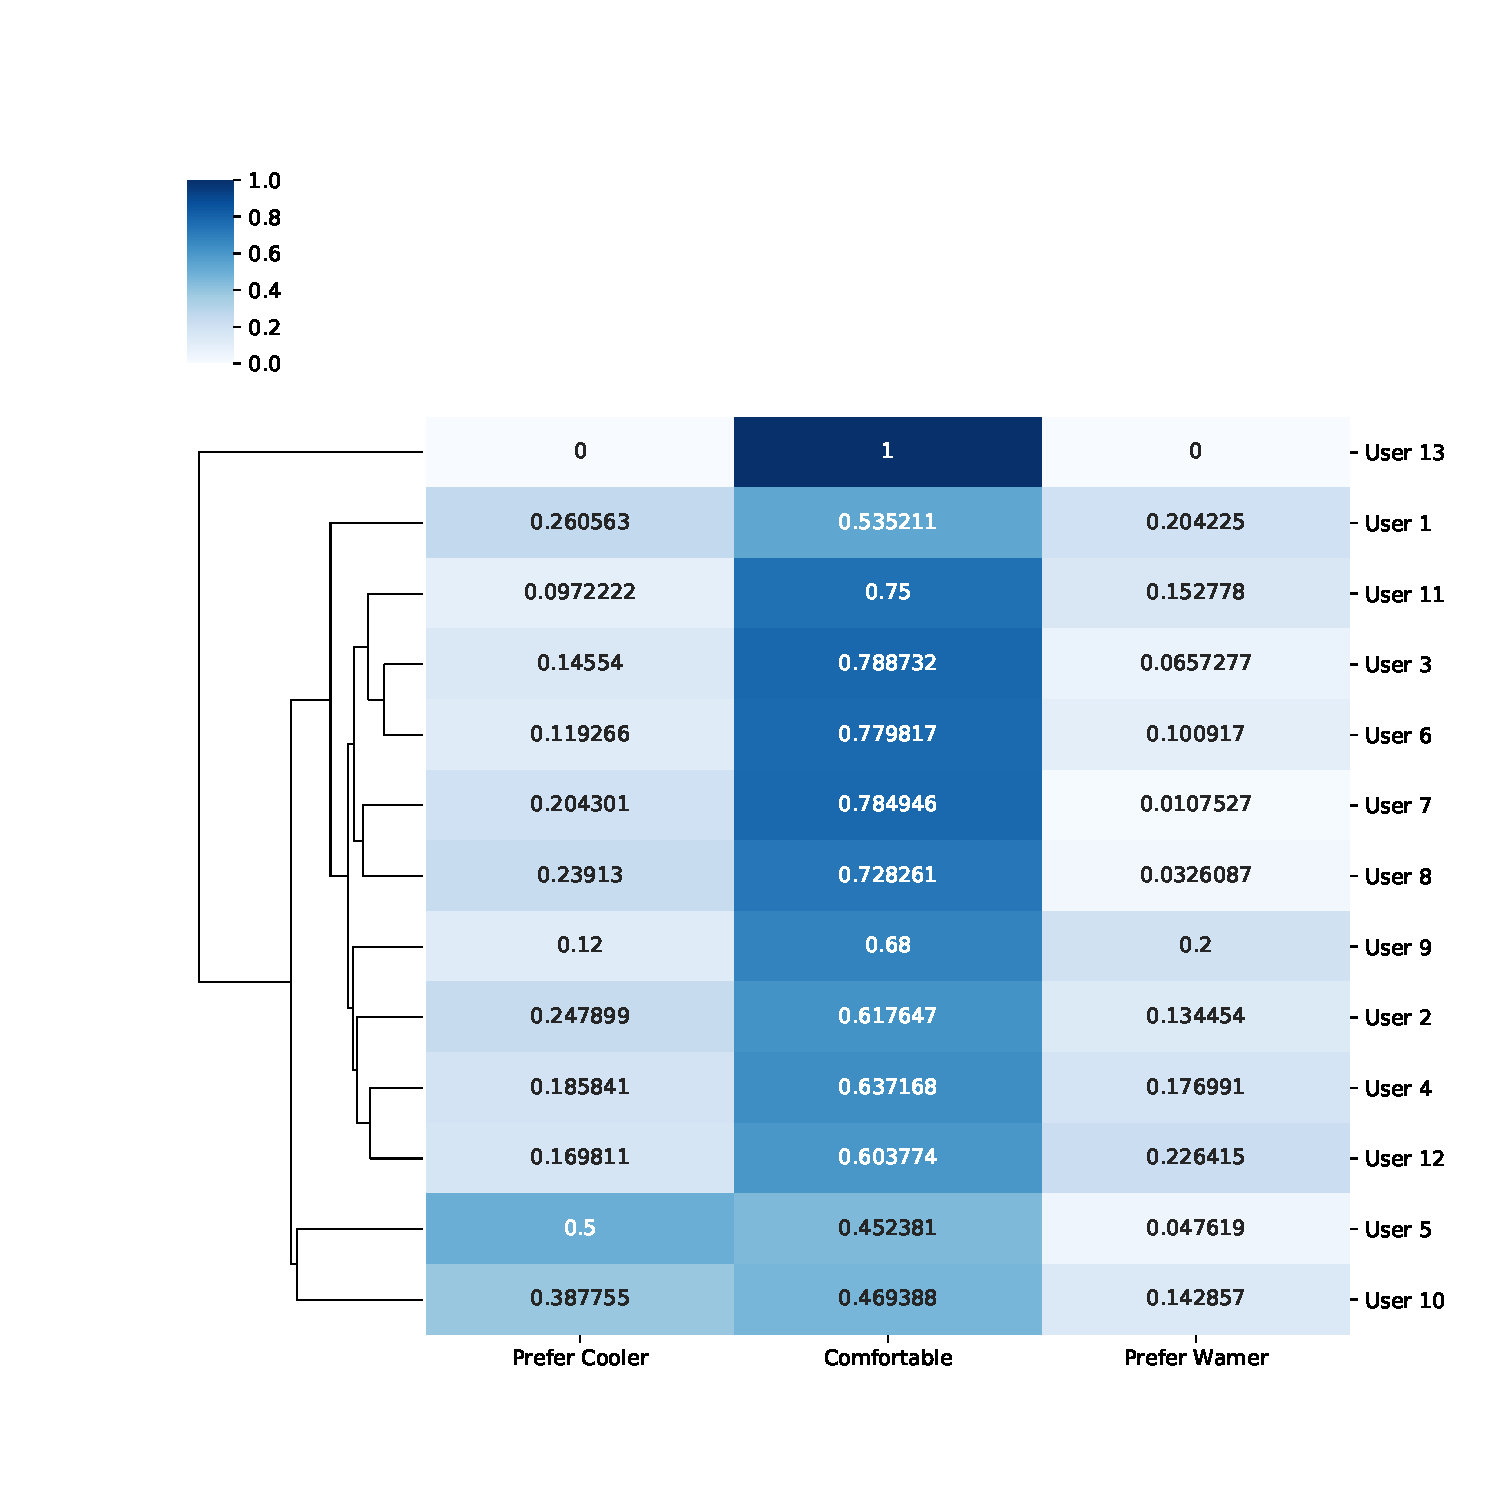
\includegraphics[width=\textwidth, trim= 0cm 0cm 0cm 0cm,clip]{cozie_users.pdf}
% 		\caption{(a)}
% 		\label{fig:userPlot}
%     \end{subfigure}
%     \begin{subfigure}[t]{0.49\textwidth}
%     \centering
%         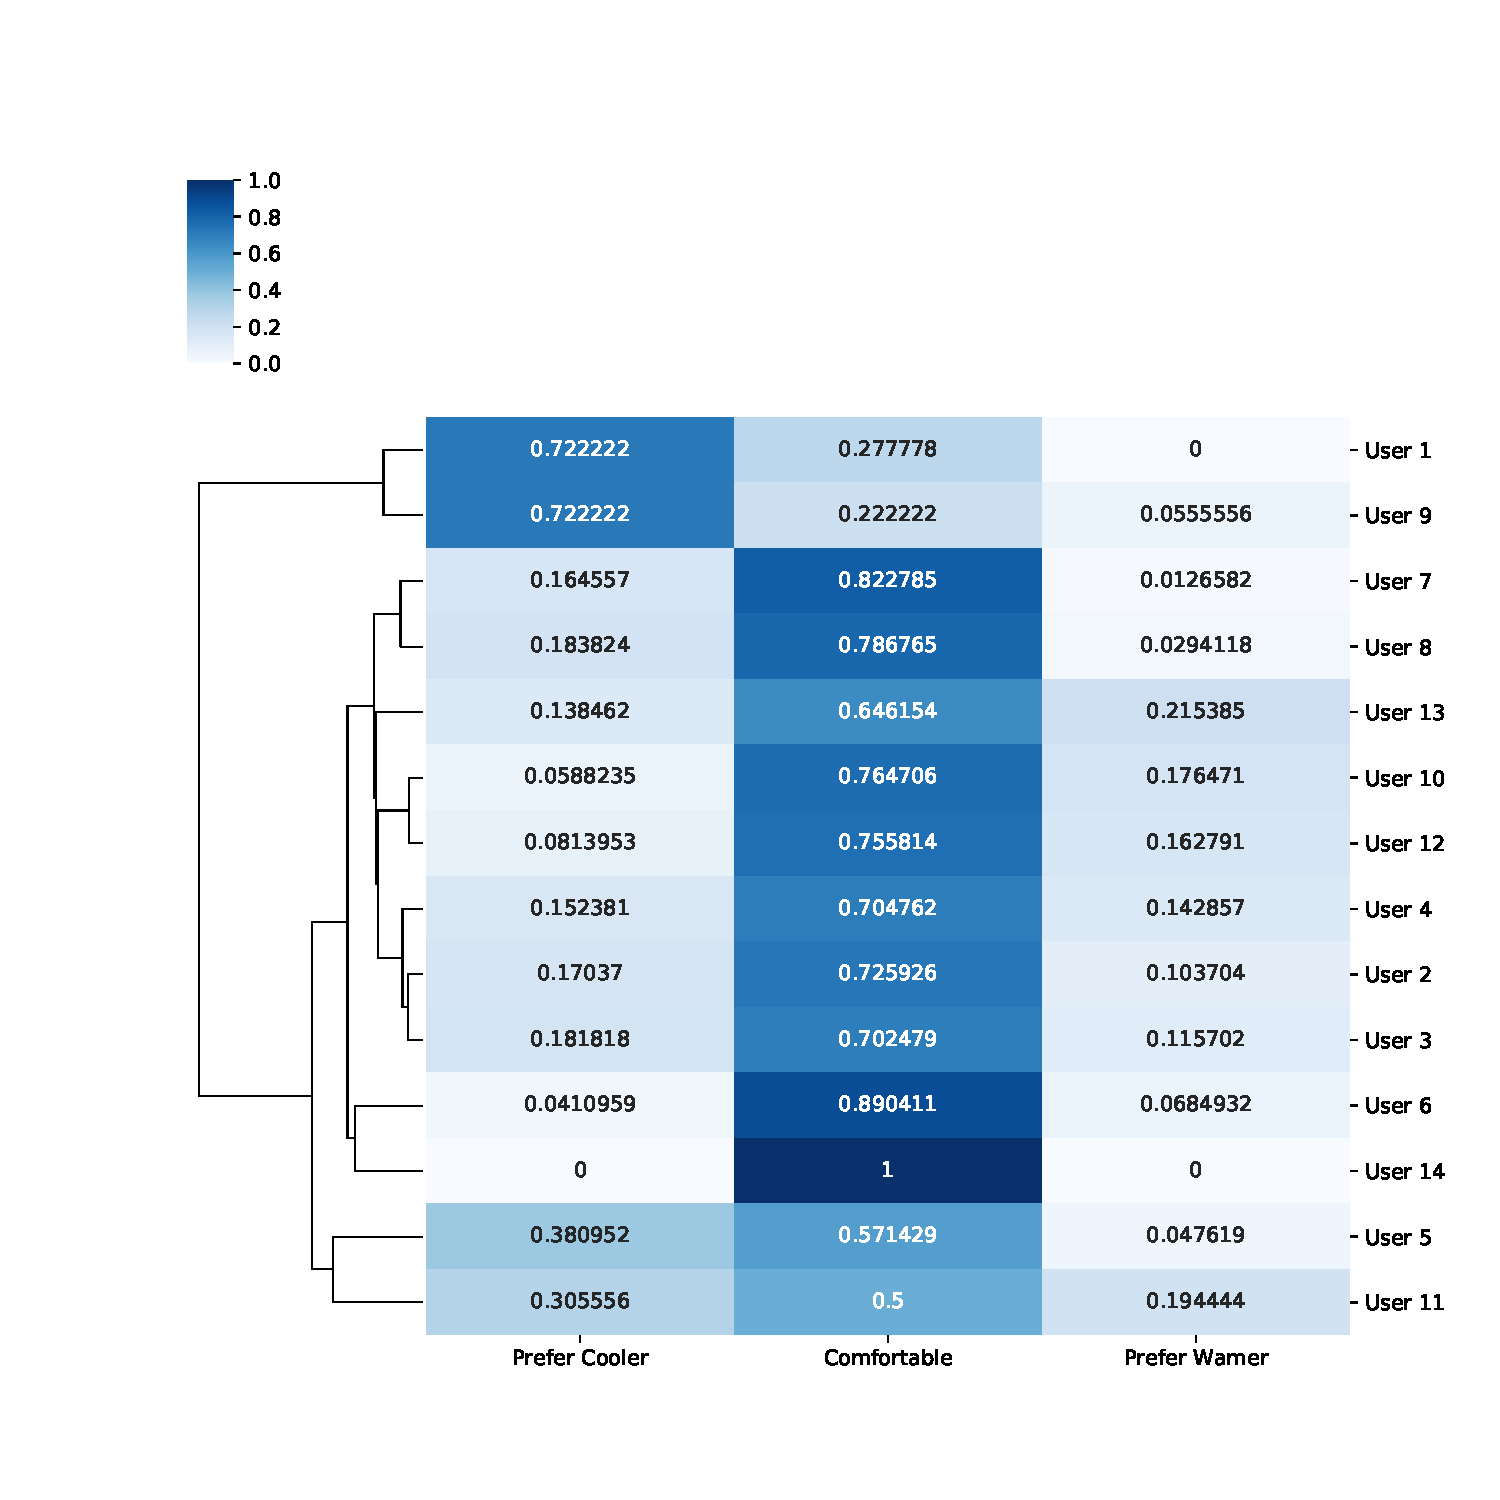
\includegraphics[width=\textwidth, trim= 0cm 0cm 0cm 0cm,clip]{cozie_users_lowheart.pdf}
% 		\caption{(b)}
% 		\label{fig:lowHeartUsers}
%     \end{subfigure}
%     \caption{Clustering of user feedback using hierarchal k-means. (a) The full results show four distinct clusters, (b) filter by heart rate that is less than 100 beats per minute}
%     \label{fig:clustering}
% \end{figure}




% \subsection{Influence of Heart-Rate}

% It is widely known that heart-rate influences metabolic activity, and therefore an occupants comfort preference. Figure \ref{fig:heartHist} details the number of responses for each thermal response based on the heart rate. [INSERT NUMBER HERE ] \% of "Prefer Cooler" responses occurred during higher metabolic activity when the heart rate was greater than 100 beats per minute. If we filter out these responses,and apply the same algorithms detailed in Section \ref{ch:userResults}, we see a slightly different response and clustering pattern, as shown in Figure \ref{fig:lowHeartUsers}. 



% \subsection{Combination with Sensor Data}




% convert time to bars
% one heart rate filter showing. Groups of similar behaving people. Group 1-4. What are the coincidental ranges of data belonging to these groups.

% \begin{figure}
% \centering
% 	\begin{subfigure}[t]{0.5\textwidth}
% 	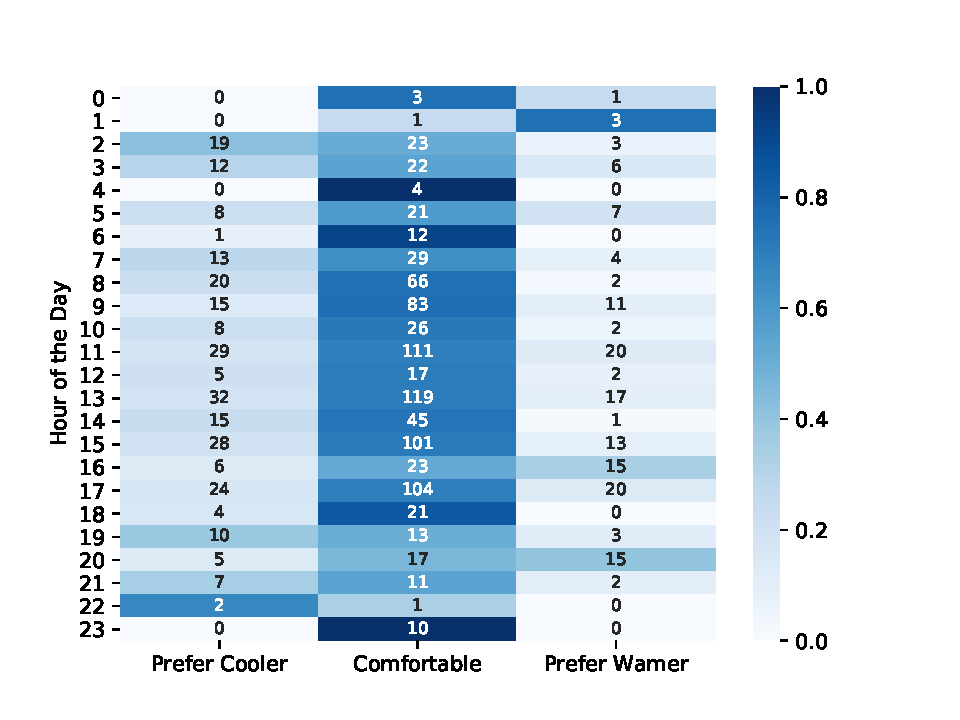
\includegraphics[width=\textwidth, trim= 0cm 0cm 0cm 0cm,clip]{hourPlot.pdf}
% 	\caption{(a)}
% 	\label{fig:hourPlot}
% 	\end{subfigure}
% 	\begin{subfigure}[t]{0.49\textwidth}
% 	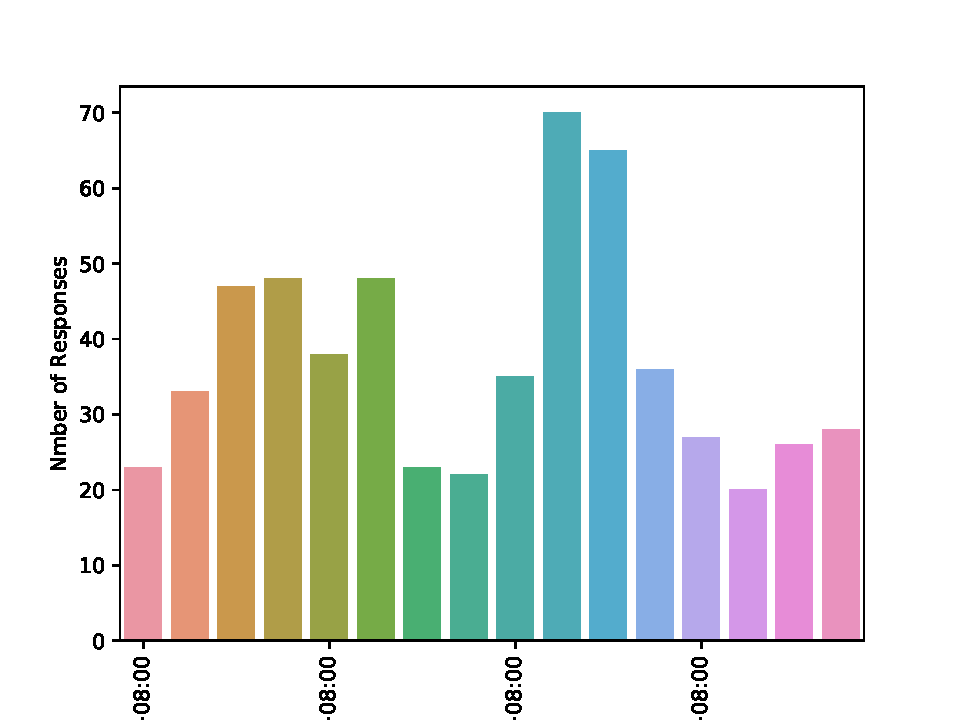
\includegraphics[width=\textwidth, trim= 0cm 0cm 0cm 0cm,clip]{response_rate.pdf}
% 	\caption{(b)}
% 	\label{fig:responseRate}
% 	\end{subfigure}
% 	\caption{(a) Aggregation of user feedback mapped to the hour of the day that feedback was given. Annotations within the heat-map detail the absolute response value, while the colour gradient relates to the normalised values (b) Daily responses during the course of the evaluation period. The dips in the graph are weekends}
% \end{figure}


% \begin{figure}
%     \centering
%     \begin{subfigure}[t]{0.3\textwidth}
%         \centering
%         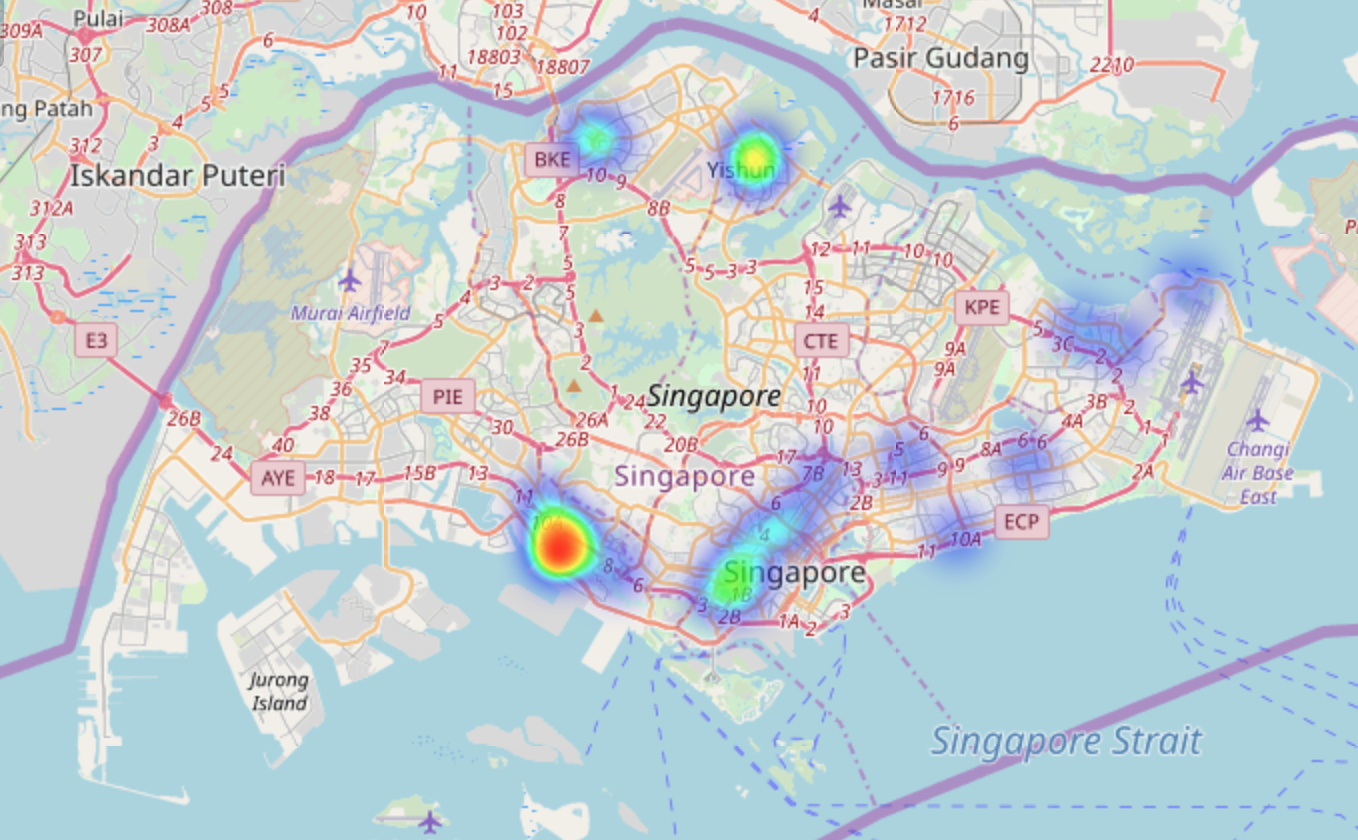
\includegraphics[height= 3cm]{map_singapore.png}
%         \caption{(a)}
%     \end{subfigure}
%     \begin{subfigure}[t]{0.3\textwidth}
%         \centering
%         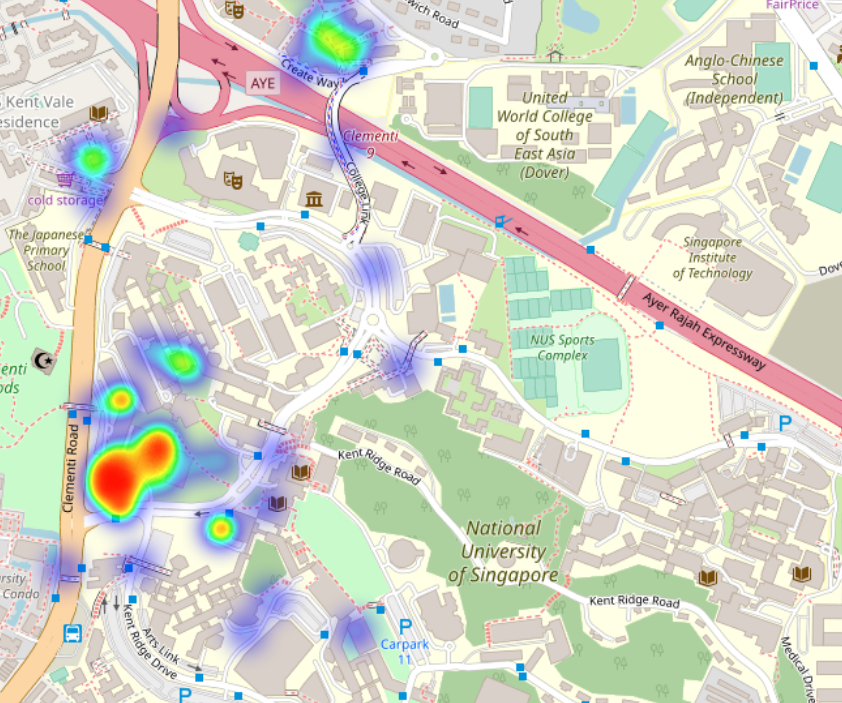
\includegraphics[height= 3cm]{map_nus.png}
%         \caption{(b)}
%     \end{subfigure}
%     \begin{subfigure}[t]{0.3\textwidth}
%         \centering
%         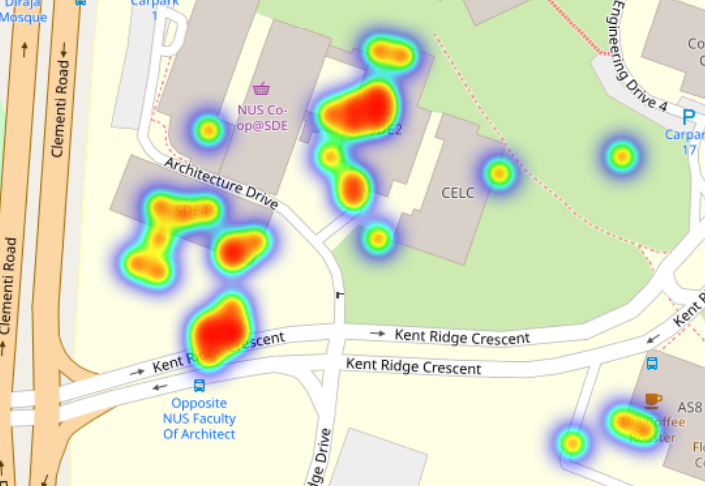
\includegraphics[height= 3cm]{map_sde.png}
%         \caption{(c)}
%     \end{subfigure}
%     \caption{Map of responses. From left to right, the city of Singapore, National University of Singapore, and the School of Design and Environment. The experiment was conducted at co-working spaces at the school of design and environment, however responses are seen throughout Singapore. Note that these results only show 634 of the [INSERT NUMBER] total responses as GPS localisation often failed indoors.}
%     \label{fig:map}
% \end{figure}



% \begin{figure}
%     \begin{subfigure}[t]{0.49\textwidth}  
%     \centering
% 	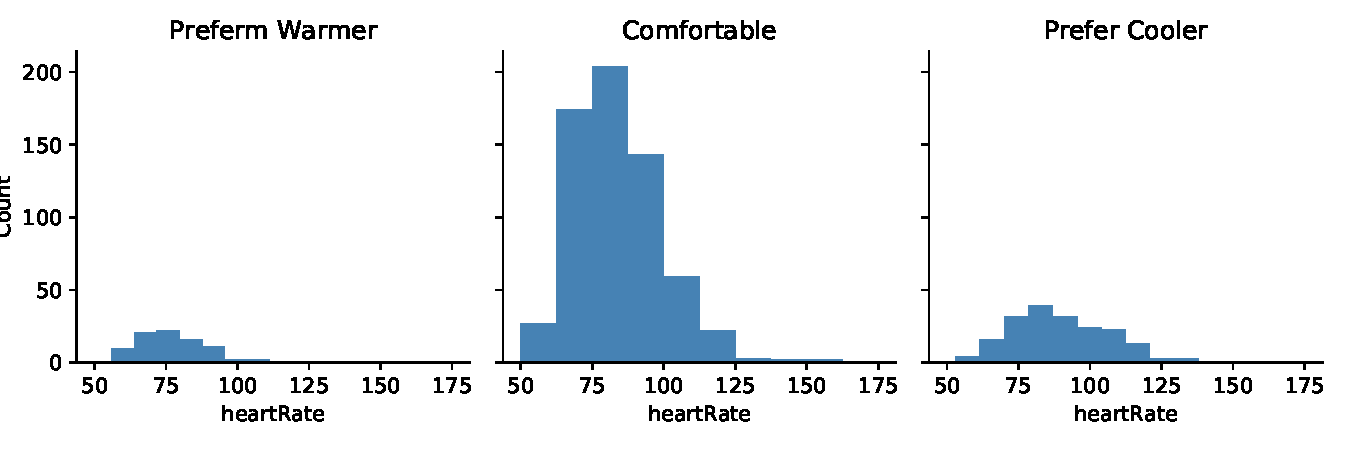
\includegraphics[width=\textwidth, trim= 0cm 0cm 0cm 0cm,clip]{heartHist.pdf}
% 	\caption{(a)}
% 	\label{fig:heartHist}
%     \end{subfigure}
%     \begin{subfigure}[t]{0.49\textwidth}
%     \centering
% 		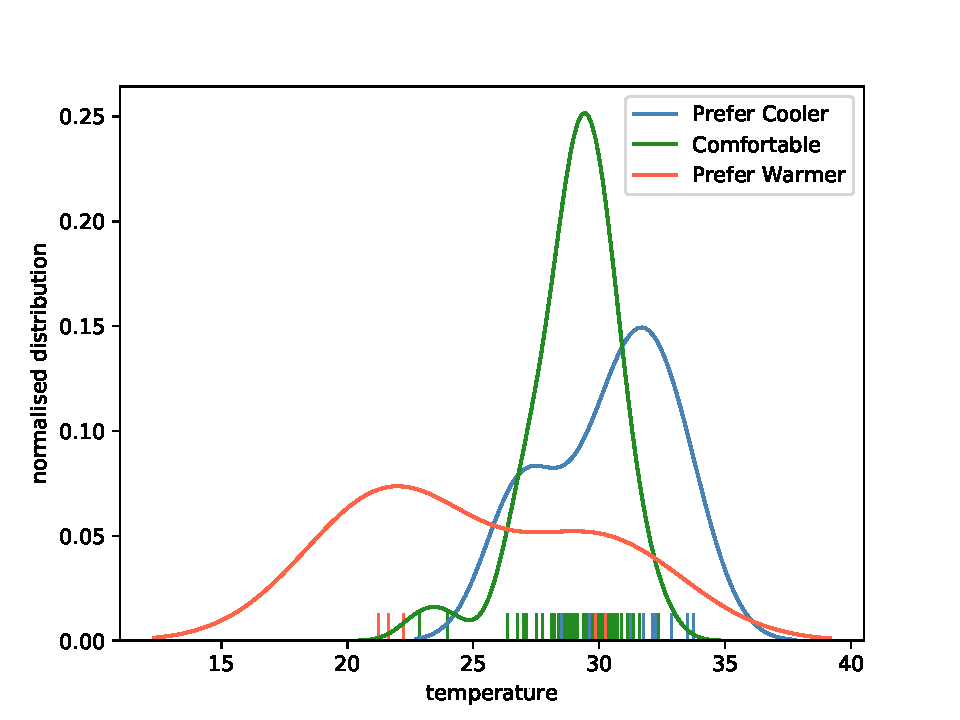
\includegraphics[width=\textwidth, trim= 0cm 0cm 0cm 0cm,clip]{temperatureHist.pdf}
% 		\caption{(b)}
% 		\label{fig:tempHist}	
%     \end{subfigure}
%     \caption{ Normalised distribution of the response type based on (a) heart rate (b) temperature. Note that the normalisation for "prefer warmer" is skewed due to the lack of responses of this type}
% \end{figure}


% \subsection{Evaluational of user comfort over a day}

% Figure \ref{fig:hourPlot} details a simple heat-map where the user comfort feedback is mapped to the hour of the day. Users appear to be comfortable on average [INSERT NUMEBR HERE] \% of the time, and there are no statistically significant trends during working hours (9:00 - 17:00). Variations in user comfort feedback during the day can be used to infer an issue within the building.

% It is interesting to note that there are more responses in the hours of 9:00, 11:00, 13:00, 15:00, and 17:00 when the occupant is buzzed and forced to give feedback. Nevertheless there are still significant amounts of responses made outside these times through the motivation of the participants themselves. Figure \ref{fig:summary}c details the daily responses from the participants, and no observable decrease in responses can be made. Dips in responses naturally occur during the weekend. 
